\icode{E-MD-MU-L3-261112-001}
（多选）
如图所示，\(A\)、\(B\) 两物块的质量分别为 \(2m\) 和 \(m\)，静止叠放在水平地面上。\(A\)、\(B\) 间的动摩擦因数为 \(\mu\)，\(B\) 与地面间的动摩擦因数为 \(\frac{1}{2}\mu\)。最大静摩擦力等于滑动摩擦力，重力加速度为 \(g\)。现对 \(A\) 施加一水平拉力 \(F\)，则\paren[]

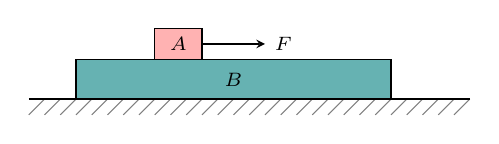
\begin{tikzpicture}[>=stealth,font=\scriptsize]
	\draw[fill=teal!60] (0,0) rectangle(4,.5)node[midway]{\(B\)};
	\draw[fill=red!30] (1,.5) rectangle(1.6,.9)node[midway]{\(A\)};
	\draw[->] (1.6,.7)--++(.8,0)node[right]{\(F\)};
	\foreach \x in {-.6,-.4,...,5}
		\draw[gray] (\x,-.2)--++(.2,.2);
	\draw[thick] (-.6,0)--(5,0);
\end{tikzpicture}
\begin{choices}
	\item 当 \(F < 2\mu mg\) 时，\(A\)、\(B\) 都相对地面静止
	\item 当 \(F = \frac{5}{2}\mu mg\) 时，\(A\) 的加速度为 \(\frac{1}{3}\mu g\)
	\item 当 \(F > 3\mu mg\) 时，\(A\) 相对 \(B\) 滑动
	\item 无论 \(F\) 为何值，\(B\) 的加速度不会超过 \(\frac{1}{2}\mu g\)
\end{choices}
\begin{answer}
	BCD\qquad 提示：
\end{answer}